\section{Results}

The results in this chapter are based data the network has not been trained with. It was also made sure that there was no overlap in images of people that were recorded multiple times. Five images were chosen randomly from each of the two sources in the very beginning. Since the Epi data featured 41 slices and the Jopp data featured 24 slices, 325 2D samples were available for evaluation. Each slice contained 50,176 pixel values, making a total of 16.3 million predictions that were analyzed.

The network architecture was developed using a single segmentation channel that merged Femur, Tibia and Fibula maps. However, tests were also run to validate the performance for each bone on its own and also combine the three separate predictions into a multi channel segmentation. The same architecture and training procedure was used for this task.

\subsection{Numeric Evaluation}

The proposed model achieves a DSC score of 98.0\% and an IoU of 96.0\%. Precision and Recall are perfectly balanced, suggesting that predictions are neither too optimistic or pessimistic. The error shows a small value of 1.2\%.

\begin{table}[H]
    \centering
    \begin{tabular}{| l | c | c | c | c | c |}
    \hline
           & DSC & IoU & Precision & Recall & Error \\ 
    \Xhline{3\arrayrulewidth}
    Merged & 0.980 & 0.960 & 0.980 & 0.980 & 0.012 \\
    \hline
    Femur & 0.981 & 0.963 & 0.979 & 0.984 & 0.006 \\
    \hline
    Tibia & 0.977 & 0.955 & 0.976 & 0.977 & 0.006 \\
    \hline
    Fibula & 0.953 & 0.911 & 0.954 & 0.952 & 0.001 \\
    \hline
    Combined & 0.979 & 0.958 & 0.977 & 0.981 & 0.004 \\
    \Xhline{3\arrayrulewidth}
    Femur \cite{Dodin2011} & 0.940 & - & - & - & - \\
    \hline
    Tibia \cite{Dodin2011} & 0.920 & - & - & - & - \\
    \hline
    Tibia \cite{Dam} & 0.975 & - & - & - & - \\
    \hline
    \end{tabular}
    \caption{Numeric evaluation of segmentations}
\end{table}

Results on Femur and Tibia alone are comparable to the merged approach, whereas the Fibula segmentation shows lower scores. This could be due to the fact that the Fibula is only visible in a minority of slices, making it a somewhat unbalanced task. Combining the three separate segmentations to a single model gives comparable results as well. The error is reduced by a factor of 3, which is expected because the channels are increased by 3. Compared to previous studies, the proposed model shows slightly better results than the multi-atlas segmentation and significantly higher scores than the ray casting technique.

\begin{figure}[H]
  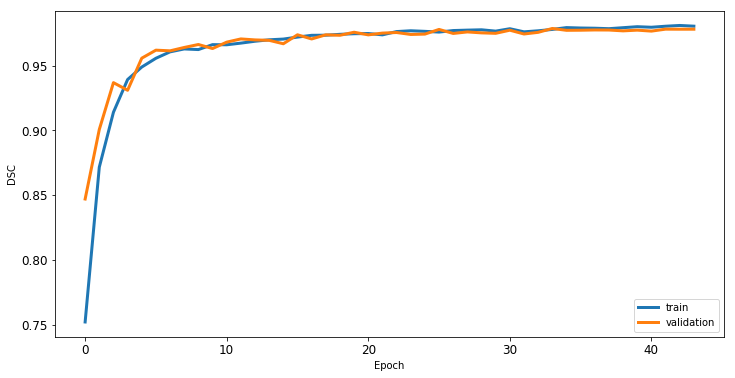
\includegraphics[width=\linewidth]{imgs/train_val.png}
\caption{Visual representation of performance during training}
\end{figure}

The graph above shows the performance of the merged model during the learning process on the training and validation data. 

\begin{table}[H]
    \centering
    \begin{tabular}{| l | c | c | c | c | c |}
    \hline
    Data       & Epoch 1 & Epoch 5 & Epoch 10 & Epoch 20 & Epoch 40 \\ 
    \Xhline{3\arrayrulewidth}
    Training Set   & 0.753   & 0.949   & 0.966    & 0.975    & 0.981 \\
    \hline
    Validation Set & 0.847   & 0.956   & 0.963    & 0.976    & 0.979 \\
    \hline
    Test Set       &     -   &     -   &     -    &     -    & 0.980 \\
    \hline
    \end{tabular}
    \caption{Performance on different sets over time}
\end{table}

The 98\% mark is never reached on the validation data, but only on the final evaluation of the test set. Towards the end the performance of the training data pulls slightly ahead of the validation results.

\subsection{Visual Evaluation}

The visual evaluation will focus on the results of the combined network since its performance is on par with the one channel model while offering more information about the associated bones.

The network shows excellent performance on slices that are located near the middle of the 3D MRIs with DSC scores of over 99\%.

\begin{figure}[H]
\minipage{0.24\textwidth}
  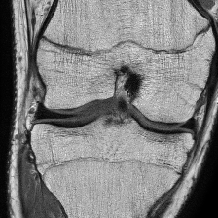
\includegraphics[width=\linewidth]{imgs/a1.png}
\endminipage\hfill
\minipage{0.24\textwidth}
  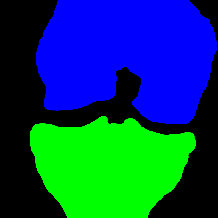
\includegraphics[width=\linewidth]{imgs/b1.png}
\endminipage\hfill
\minipage{0.24\textwidth}%
  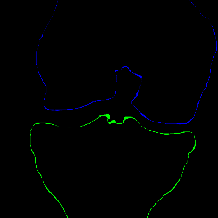
\includegraphics[width=\linewidth]{imgs/c1.png}
\endminipage\hfill
\minipage{0.24\textwidth}%
  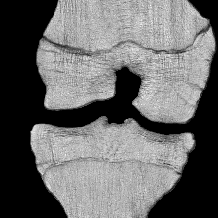
\includegraphics[width=\linewidth]{imgs/d1.png}
\endminipage
\vspace{0.15cm}
\minipage{0.24\textwidth}
  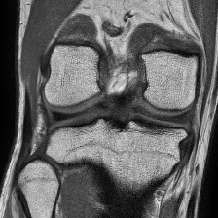
\includegraphics[width=\linewidth]{imgs/a2.png}
\endminipage\hfill
\minipage{0.24\textwidth}
  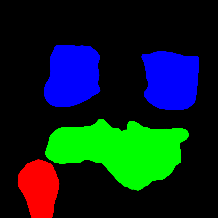
\includegraphics[width=\linewidth]{imgs/b2.png}
\endminipage\hfill
\minipage{0.24\textwidth}%
  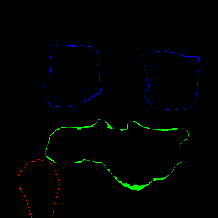
\includegraphics[width=\linewidth]{imgs/c2.png}
\endminipage\hfill
\minipage{0.24\textwidth}%
  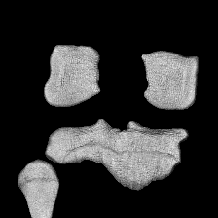
\includegraphics[width=\linewidth]{imgs/d2.png}
\endminipage
\vspace{0.15cm}
\minipage{0.24\textwidth}
  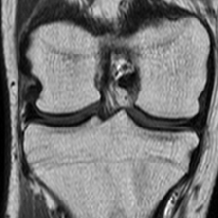
\includegraphics[width=\linewidth]{imgs/a3.png}
\endminipage\hfill
\minipage{0.24\textwidth}
  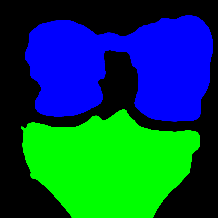
\includegraphics[width=\linewidth]{imgs/b3.png}
\endminipage\hfill
\minipage{0.24\textwidth}%
  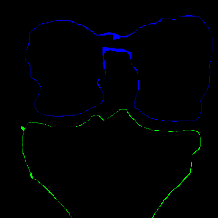
\includegraphics[width=\linewidth]{imgs/c3.png}
\endminipage\hfill
\minipage{0.24\textwidth}%
  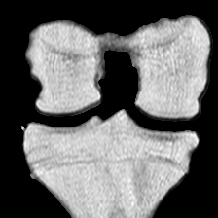
\includegraphics[width=\linewidth]{imgs/d3.png}
\endminipage
\vspace{0.15cm}
\minipage{0.24\textwidth}
  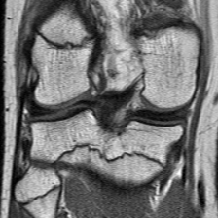
\includegraphics[width=\linewidth]{imgs/a4.png}
\endminipage\hfill
\minipage{0.24\textwidth}
  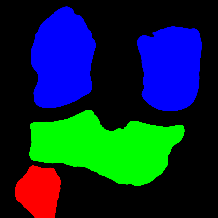
\includegraphics[width=\linewidth]{imgs/b4.png}
\endminipage\hfill
\minipage{0.24\textwidth}%
  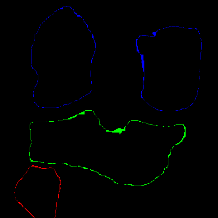
\includegraphics[width=\linewidth]{imgs/c4.png}
\endminipage\hfill
\minipage{0.24\textwidth}%
  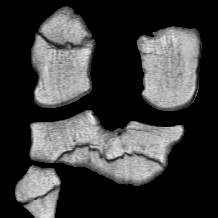
\includegraphics[width=\linewidth]{imgs/d4.png}
\endminipage
\caption{Input, prediction, difference to ground truth and applied mask}
\end{figure}

Perfect DSC scores of 100\% are achieved through empty segmentations that the network correctly predicted as such.

\begin{figure}[H]
\minipage{0.24\textwidth}
  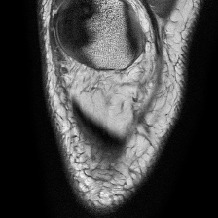
\includegraphics[width=\linewidth]{imgs/a5.png}
\endminipage\hfill
\minipage{0.24\textwidth}
  
\includegraphics[width=\linewidth]{imgs/b5.png}
\endminipage\hfill
\minipage{0.24\textwidth}%
  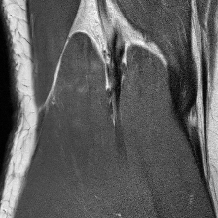
\includegraphics[width=\linewidth]{imgs/a6.png}
\endminipage\hfill
\minipage{0.24\textwidth}%
  
\includegraphics[width=\linewidth]{imgs/b6.png}
\endminipage
\caption{Correctly segmented upper and lower slices}
\end{figure}

The most imprecise predictions also appeared in upper and lower slices where the bones started to become visible. If either the prediction or the ground truth was empty while the other was not, then the result is a DSC score of 0\%.

\begin{figure}[H]
\minipage{0.32\textwidth}
  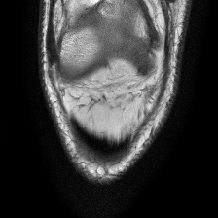
\includegraphics[width=\linewidth]{imgs/a8.png}
\endminipage\hfill
\minipage{0.32\textwidth}
  
\includegraphics[width=\linewidth]{imgs/b8.png}
\endminipage\hfill
\minipage{0.32\textwidth}%
  
\includegraphics[width=\linewidth]{imgs/c8.png}
\endminipage
\vspace{0.2cm}
\minipage{0.32\textwidth}
  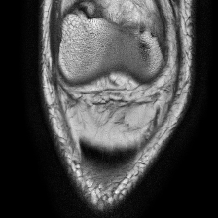
\includegraphics[width=\linewidth]{imgs/a7.png}
\endminipage\hfill
\minipage{0.32\textwidth}
  
\includegraphics[width=\linewidth]{imgs/b7.png}
\endminipage\hfill
\minipage{0.32\textwidth}%
  
\includegraphics[width=\linewidth]{imgs/c7.png}
\endminipage
\caption{Input, ground truth and prediction of false segmentations}
\end{figure}

In these examples, the ground truth defines the Femur to be visible in the upper image but not in the one below it. The prediction disagrees with it in both cases. These are two examples that could be seen as noise in the ground truth data or to be debatable at least.

\subsection{Model Exploration}

Neural networks are often considered black boxes because it is difficult to get an intuitive understanding how decisions are calculated. This is a crucial problem especially in the medical field, where a prediction may approximate certain health conditions about a patient.

Two factors help in this study to pull away from this problem. Firstly, a segmentation is an image to image pipeline making it less abstract what kind of transformations are happening. Visualizing input and output gives an intuitive understanding how one may have emerged out of the other.

Secondly, convolutional neural networks take away most of this black box reasoning \cite{Chollet2017} because every layer in the network can be visualized. The following images give an insight what a sample looks like after different convolutional blocks.

\begin{figure}[H]
  \centering
  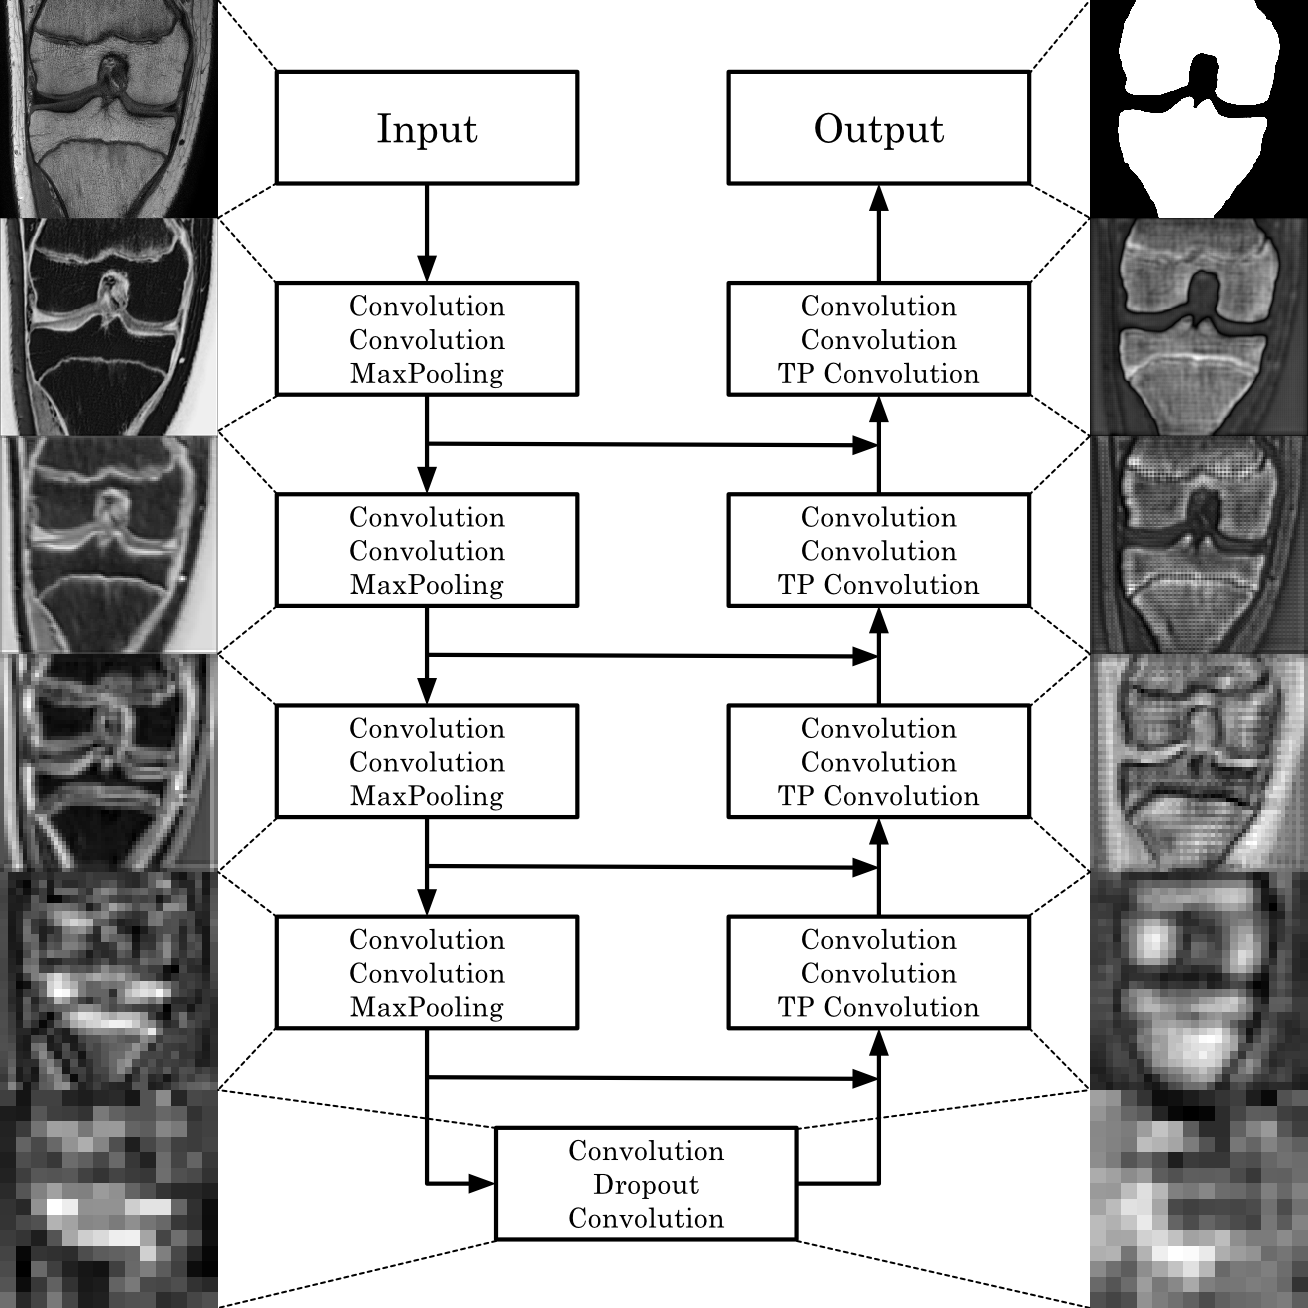
\includegraphics[width=0.95\textwidth]{imgs/archi_explo.png}
\caption{Intermediate sum of feature maps throughout the network}
\end{figure}

Each image shows the sum of all intermediate channels at a particular layer. The first image is the raw input, whereas the last image is the final segmentation map. One can clearly see the reduction of resolution towards the middle, which is then brought back up. The first convolutional block inverses the input and removes most of the bone structure except for the growth plates. The second to last output looks similar to the input, but the skin on the sides is almost entirely removed, and the dark growth plates have been filled. Looking closer at this image one can also notice a crisp black line that separates the bone from the rest. A simple threshold at this point would segment the bone fairly accurate.

Even at this level, it is difficult to judge what exactly the network is detecting. For another visualization, the intermediate channels are not added like before but analyzed separately.

\begin{figure}[H]
\minipage{0.24\textwidth}
  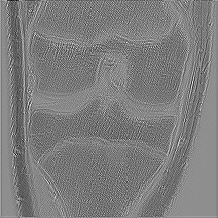
\includegraphics[width=\linewidth]{imgs/channel1.png}
\endminipage\hfill
\minipage{0.24\textwidth}
  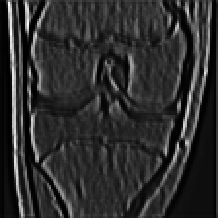
\includegraphics[width=\linewidth]{imgs/channel3.png}
\endminipage\hfill
\minipage{0.24\textwidth}%
  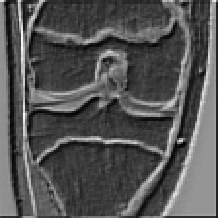
\includegraphics[width=\linewidth]{imgs/channel2.png}
\endminipage\hfill
\minipage{0.24\textwidth}%
  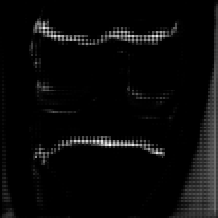
\includegraphics[width=\linewidth]{imgs/channel4.png}
\endminipage
\caption{Examples of intermediate channels throughout the network}
\end{figure}

These are a few notable examples inside the model. The first filter detects high frequencies in the bone and skin tissue. Filter 2 finds vertical edges while filter 3 shows horizontal ones. Finally, filter 4 appears to be a growth plate detector. It does not just detect horizontal edges, but only those inside the bone. This seems reasonable because the network needs to learn that the dark growth plates shouldn't be interpreted as edges.

\subsection{Noise Exploitation}

Ground truth data is often subject to noise, because mistakes happen during their creation or because it may be debatable what the actual truth is. To test how well the network performs on noisy data, another training environment was set up where synthetic noise was added to the ground truth segmentations. By using erosion and dilation with a kernel size of 7 both the training and validation sets were modified.

\begin{figure}[H]
\minipage{0.24\textwidth}
  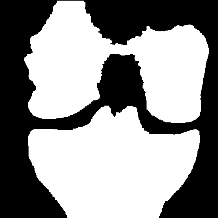
\includegraphics[width=\linewidth]{imgs/orig_seg1.png}
\endminipage\hfill
\minipage{0.24\textwidth}
  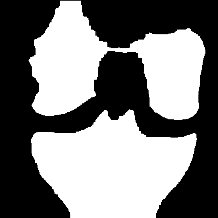
\includegraphics[width=\linewidth]{imgs/noisy_seg1.png}
\endminipage\hfill
\minipage{0.24\textwidth}%
  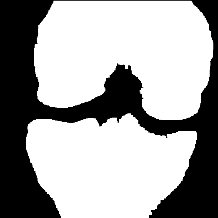
\includegraphics[width=\linewidth]{imgs/orig_seg2.png}
\endminipage\hfill
\minipage{0.24\textwidth}%
  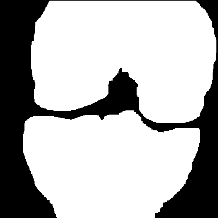
\includegraphics[width=\linewidth]{imgs/noisy_seg2.png}
\endminipage
\caption{Examples of synthetic noise}
\end{figure}

The first and third images show the original segmentations, while 2 and 4 were changed using erosion and dilation respectively. The noise on the training data accounted for an error of 7.1\% DSC. Afterward, the unmodified test data was loaded to verify the results. The predictions show an accuracy of 95.2\% DSC, meaning that the noise hurts the performance of the model.

More importantly however, the DSC error is lower than the error that was introduced through the noise in the training data. When applying the same noise on the test set and using it as a prediction for the actual ground truth, the score is 92.8\% DSC. The predictions of the network contain 33\% less noise than the data it was trained on.

\subsection{Transfer Application}

Neural networks are known to be unreliable when used on data that exceeds the range of variation in the training set. They cannot learn what they weren't taught. On the other hand, convolutions are translation invariant, allowing them to recognize patterns anywhere in the frame \cite{Chollet2017}. Another merged model was trained that used the same architecture but added further image augmentation of horizontal and vertical flips. This way it only reached a DSC score of 97.3\% but was more flexible to structural differences in the image.

The proposed architecture can be described as "fully convolutional" because it doesn't include any dense layers. This allows the network to accept any resolution and still being able to process it. An experiment was set up that used uncropped images from the Epi data which were resized to 448x448 pixels. This made them four times larger than the images the network was trained with.

\begin{figure}[H]
\minipage{0.24\textwidth}
  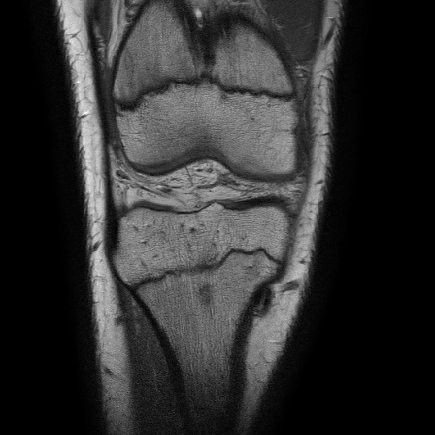
\includegraphics[width=\linewidth]{imgs/transfer_size_x1.png}
\endminipage\hfill
\minipage{0.24\textwidth}
  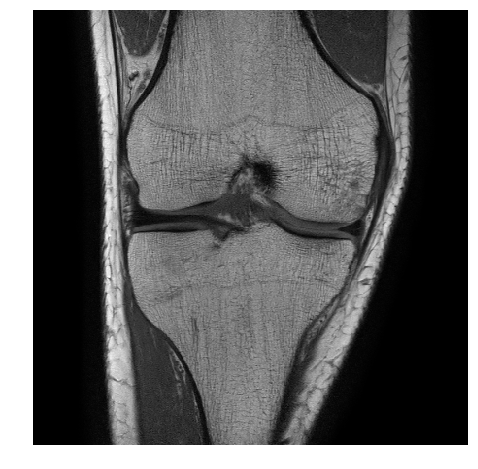
\includegraphics[width=\linewidth]{imgs/transfer_size_x2.png}
\endminipage\hfill
\minipage{0.24\textwidth}%
  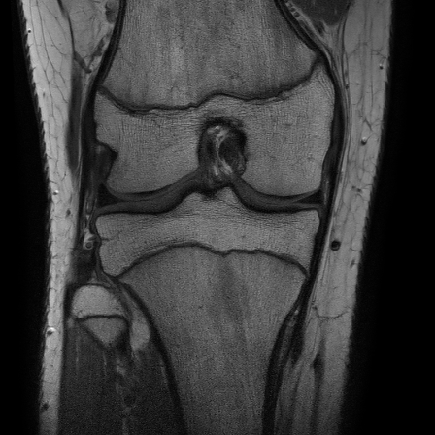
\includegraphics[width=\linewidth]{imgs/transfer_size_x3.png}
\endminipage\hfill
\minipage{0.24\textwidth}%
  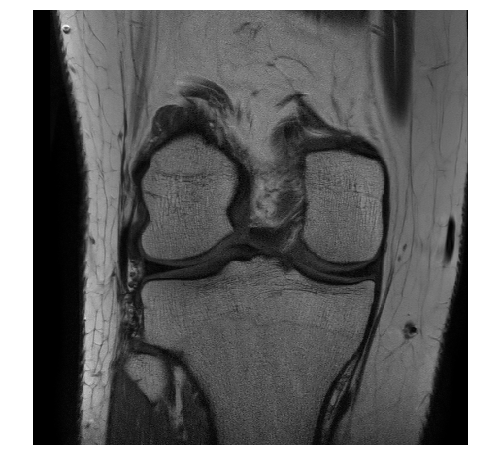
\includegraphics[width=\linewidth]{imgs/transfer_size_x4.png}
\endminipage
\vspace{0.15cm}
\minipage{0.24\textwidth}
  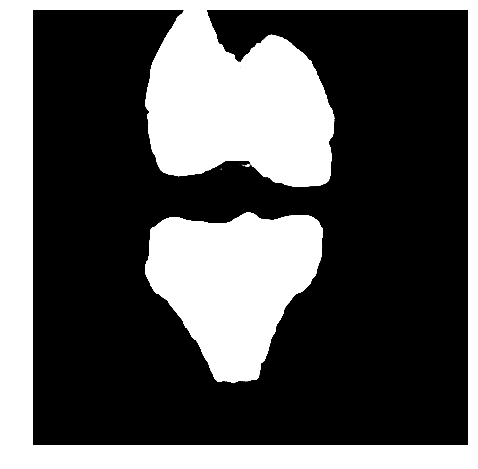
\includegraphics[width=\linewidth]{imgs/transfer_size_y1.png}
\endminipage\hfill
\minipage{0.24\textwidth}
  
\includegraphics[width=\linewidth]{imgs/transfer_size_y2.png}
\endminipage\hfill
\minipage{0.24\textwidth}%
  
\includegraphics[width=\linewidth]{imgs/transfer_size_y3.png}
\endminipage\hfill
\minipage{0.24\textwidth}%
  
\includegraphics[width=\linewidth]{imgs/transfer_size_y4.png}
\endminipage
\caption{Examples of uncropped and 448x448 pixel predictions}
\end{figure}

The predictions show good results even following the shaft of the bone which wasn't visible in the original cropped images. Even large intensity gaps through growth plates are recognized as Femur or Tibia. The recall performance is very accurate. Problems are visible in tissue that isn't bone but was recognized as such as the 4th examples shows.

In 3.2 a third data source was mentioned that featured five sagittal recordings of knees. These were not used for the training because of their structural differences and because no ground truth segmentations were available. The following samples show what happens when the network is applied to images from a different perspective.

\begin{figure}[H]
\minipage{0.24\textwidth}
  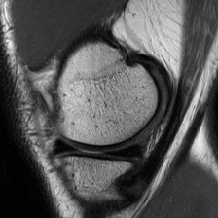
\includegraphics[width=\linewidth]{imgs/transfer_pers_x1.png}
\endminipage\hfill
\minipage{0.24\textwidth}
  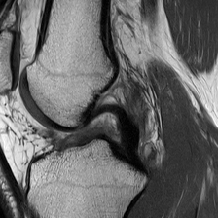
\includegraphics[width=\linewidth]{imgs/transfer_pers_x2.png}
\endminipage\hfill
\minipage{0.24\textwidth}%
  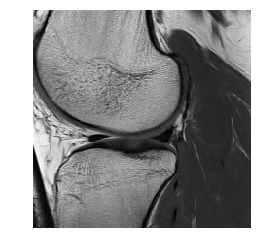
\includegraphics[width=\linewidth]{imgs/transfer_pers_x3.png}
\endminipage\hfill
\minipage{0.24\textwidth}%
  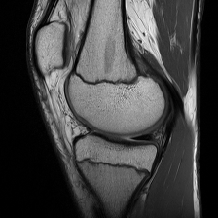
\includegraphics[width=\linewidth]{imgs/transfer_pers_x4.png}
\endminipage
\vspace{0.15cm}
\minipage{0.24\textwidth}
  
\includegraphics[width=\linewidth]{imgs/transfer_pers_y1.png}
\endminipage\hfill
\minipage{0.24\textwidth}
  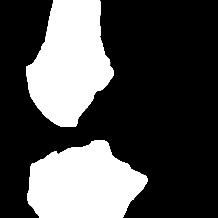
\includegraphics[width=\linewidth]{imgs/transfer_pers_y2.png}
\endminipage\hfill
\minipage{0.24\textwidth}%
  \includegraphics[width=\linewidth]{imgs/transfer_pers_y3.png}
\endminipage\hfill
\minipage{0.24\textwidth}%
  \includegraphics[width=\linewidth]{imgs/transfer_pers_y4.png}
\endminipage
\caption{Examples of sagittal class 3 data segmentations}
\end{figure}

These results look very accurate. In example 4 it even recognizes the Patella, a bone it was never trained on. This shows that with enough image augmentation the network will learn to segment any bone.

\subsection{Age Assessment}

The initial cause for the segmentation experiment was to reduce the amount of information in a knee MRI. The resulting images could then be used to make age assessments that focussed on the bone and the growth plate. This section will briefly cover such an age prediction pipeline.

The age of the candidates ranged from 14 to 21 years with a mean at 17.5 years. Predicting this age for every person meant that it was never off more than 3.5 years. Since the data was normally distributed, a static prediction of the mean led to a mean absolute error (MAE) of 1.2 years.

Even by using many of the techniques mentioned in previous chapters, it was not possible to train a stable model that could beat this baseline on the raw input data. After the segmentation maps had been applied to all 145 3D samples, many of the slices were completely empty because they didn't contain any of the three bones. It was decided to only use the middle 18 slices from each of the two sources. Even with these changes the network wouldn't converge.

Only after using the contracting side of the proposed model with the parameters it learned on the segmentation task was it possible to train a network in a stable manner. This approach did not make the model converge every time, but when it did its predictions were stable through multiple epochs.

The results on the test data showed an MAE of 0.66 years for all of the slices. Since every 3D sample now had 18 different predictions, another tree based model was built that would take a vector of 18 values and predict a single age. This got a final MAE of 0.55 years on the test data, which is more than twice as good as the baseline.

\newpage